\documentclass{article}

\usepackage[margin=1in]{geometry}
\usepackage{graphicx}
\usepackage{listings}
\usepackage{siunitx}
\usepackage{float}

\begin{document}



\begin{table}[h]
\begin{center}
\label{code:resis}
\begin{tabular}{c|c|c|c}
Variable	&	Calculated value	&	Measured Value	&	Percent Difference	\\\hline
$V_T$	&	16.276	[V] &	16.29	[V] &	0.086	\% \\
$I_N$	&	50.21	[mA] &	49.31	[mA] &	1.7925	\% \\
$R_T$	&	324.178	$\Omega$ &	330.35	$\Omega$ &	1.9039	\% \\
$R_N$	&	324.178	$\Omega$ &	330.35	$\Omega$ &	1.9039	\% \\

\end{tabular}
\end{center}

\end{table}

\pagebreak


\begin{table}[h]
\begin{center}
\label{code:resis}
\caption{Lab 5 Comparisons}
\begin{tabular}{c|c|c|c|c|c|c|c}
 Nominal $R_L$	&	$R_L$	&	Calc. $V_L$	& $V_L$	&	Calc. $I_L$	&	$I_L$	&	Calc.  $P_L$	&	$P_L$	\\\hline
$100	\Omega$ &	$98.2	\Omega$ &	3.78708	[V] &	3.3727	[V] &	37.8708	[mA] &	38.04	[mA] &	143.420	[mW] &	128.298	[mW] \\
$1000	\Omega $&	$985	\Omega$ &	12.2478	[V] &	12.23	[V] &	12.2478	[mA] &	12.1	[mA] &	150.009	[mW] &	147.983	[mW] \\


\end{tabular}
\end{center}

\end{table}

\begin{figure}[h]
  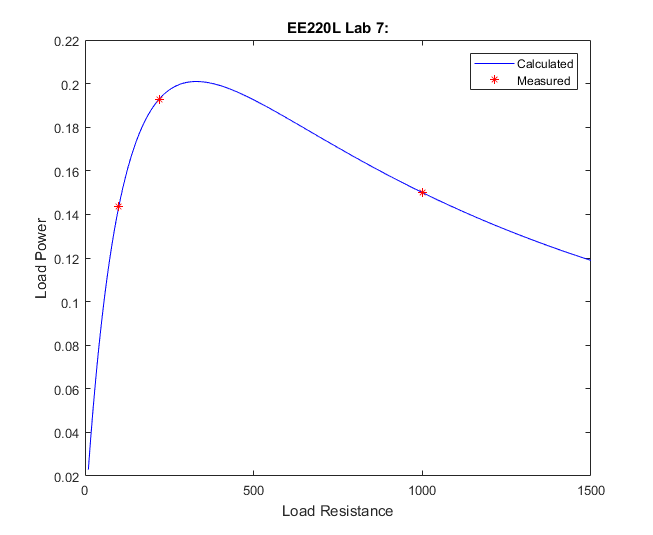
\includegraphics[width=4in]{lab7.png}
  \caption{Power vs Resistance}
  \label{fig:4a}
\end{figure}




\lstinputlisting[caption={MATLAB code for Lab 7 Circuits 1},
 label={code:lab_7}, frame=tb]{Lab7_anal.m}

\begin{lstlisting}

\end{lstlisting}

\end{document}
